%---------- COURSE INFORMATION ------------------------
\newcommand{\course}{CIS 430-01}
\newcommand{\coursetitle}{SPECIAL TOPICS - ADVANCED PROGRAMMING TECHNIQUES WITH \\ \hspace*{.4in}PYTHON}
\newcommand{\courseloc}{Raburn 210}
\newcommand{\coursetime}{Tuesday/Thursday 9:30 p.m. - 10:45 a.m.}
\newcommand{\coursedesc}{Select topics varying according to the need and interest of students. Prerequisite: approval of instructor. (Offered on sufficient demand)}
\newcommand{\coursesec}{01}
\newcommand{\coursecredithours}{3}
\newcommand{\courseprereq}{CIS 225 or CS 155 (with a grade of ``C'' or higher)}
\newcommand{\coursedelmethod}{Traditional Classroom}

\newcommand{\courseobjectives}{
	\item Improve creating basic computer programs in Python [CIS Program Outcome a][COB Goals 2,3].
	\item Explain programming theory related to pythong [CIS Program Outcomes a,b,i][COB Goal 3].
	\item Use complex python application programming interfaces (APIs) to [CIS Program Outcomes a,b,i][COB Goal 3]:
	\begin{enumerate}
		\item create a data-driven web application
		\item create a graphical user interface
		\item create a geographic information systems (GIS) program to perform advanced functions or automate common GIS tasks
	\end{enumerate}
	\item Develop mechanisms for accessing relational databases from various types of application development environments [CIS Program Outcomes a,b,c,i] [COB Goal 3].
	\item Develop object-oriented programs using python [CIS Program Outcomes a,b,i][COB Goal 3].
	\item Explain object-oriented programming concepts [CIS Program Outcomes a,b,i][COB Goal 3].
	\item Communicate and work in teams [CIS Program Outcome d][COB Goal 1].
	\item Engage in continuing professional development [CIS Program Outcome h][COB Goals 3,4].
}

\newcommand{\coursetopics}{
	\item Python programming basics
	\item Object-oriented python concepts
	\item Using python APIs
	\item Programming graphical user interfaces with python toolkits
	\item Programming web-based applications
	\item Programming GIS applications using python scripts
}
\newcommand{\coursegrades}{
	Subject exams (2 exams @ 10\% each)\dotfillsmall 20\% \\
	Project work\dotfillsmall 20\% \\
	Final project (presentation and artifacts)\dotfillsmall 30\% \\
	Final exam\dotfillsmall 30\%
}
\newcommand{\coursetext}{
	\adjustbox{valign=c}{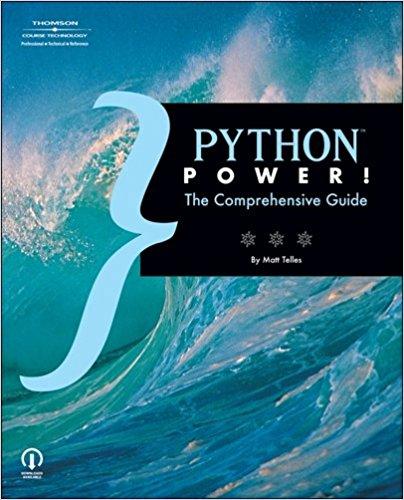
\includegraphics[width=1in]{img/cis430-1}} & \hangindent .4in \textbf{Textbook:} Tellez, M., Python Power!: The Comprehensive Guide (1st Edition). Cengage Learning PTR. ISBN-13: 978-1598631586 $\bullet$ ISBN-10: 1598631586. \\
	\\
	\adjustbox{valign=c}{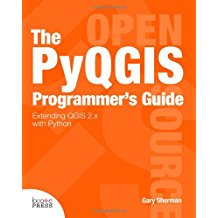
\includegraphics[width=1in]{img/cis430-2}} & \hangindent .4in \textbf{Textbook:} Sherman, G. (2014). The Pyqgis Programmer's Guide. Locate Press. ISBN-10: 0989421724 $\bullet$ ISBN-13: 978-0989421720. 
	%& \hangindent .4in Simulation Software: SAM 365 \& 2016 Assessments, Trainings, and Projects with MindTap Reader.
}